In this chapter I will give an overview of applications within branches of music information retrieval that are related to music structure analysis. Two machine learning architectures are introduced. Then previous work of the distance-based segmentation and annotation approach is reviewed and the current state-of-the-art to music structure analysis is showed. This chapter ends with an overview of datasets and acoustic features that can be used for music structure analysis. 


\section[ML in MIR]{Machine learning in Music Information\\Retrieval}
Although machine learning has not been applied on a wide scale to the SbA approach to \msa, it is already being used and researched upon within \mir\ (MIR) and music generation. Because \mir\ involves many disciplines regarding music that extend well beyond the scope of this thesis, as does music generation, I will focus on applications of machine learning closely related to \msa. See \citetitle{Muller} \cite{Muller} for an extensive introduction to basis and main disciplines of \mir.

\subsection[ML for AAS]{Machine Learning for \aas}
\begin{figure}[t]
    \centering
    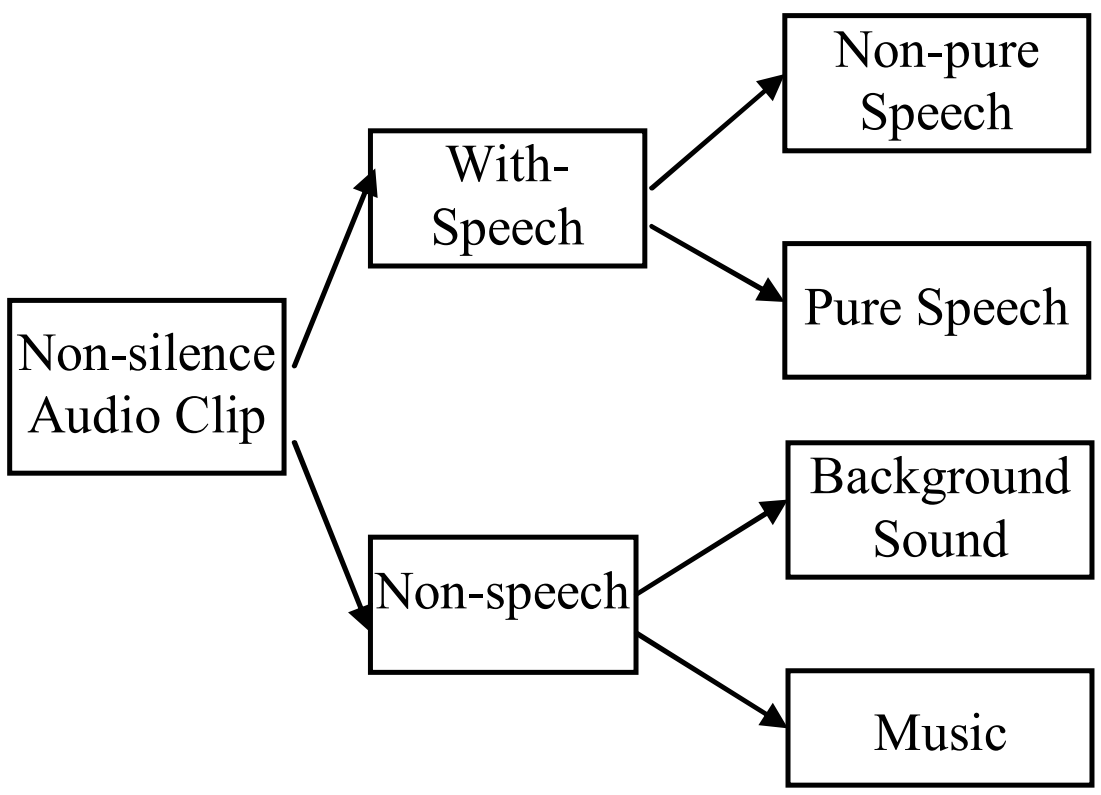
\includegraphics[width=0.5\textwidth]{images/broadcast_classification}
    \caption{Example multi-class classification tree for multi-class broadcast domain data classification or \textit{Automatic Audio Segmentation}.\\
    Reprinted from \textcite{Lu2001content} (Figure 2)}
    \label{fig:broadcast_classification}
\end{figure}
One of the fields in which machine learning has been (successfully) applied, is classifying pieces of audio in an audio stream. The classes to be distinguished are \textit{speech}, \textit{music} and various kinds of \textit{background noises} or \textit{silence}. Each class can be made as specific as desired; one could be interested in finding only the parts within an audio stream where the same person is talking, or where only music is played. This is often referred to as \textit{Automatic Audio Segmentation} (AAS). 

\textcite{Theodorou2014overview} gives an overview of different approaches and implementations to automatic audio segmentation. They describe a distance-based approach similar to the distance-based segmentation and annotation approach to MSA. One of the downsides of this approach is that it does not classify each segment, because it is limited to solely finding the segment boundaries. One other approach they describe is the \sba\ approach. Within automatic audio segmentation, this approach works in a similar way as the SbA approach to music structure analysis, by subdividing an audio stream into small pieces and assigning a class to each small piece. \citeauthor{Theodorou2014overview} mention this approach as being specifically suited for machine learning, because of the high performance of machine learning models on classification problems.

First uses of machine learning used for automatic audio segmentation used machine learning methods that did not employ deep learning, such as Gaussian Mixture Models \cite{Misra2012speech,Kos2009line,Zhang2010audio,Butko2011audio,Dogan2009content}, Support Vector Machines \cite{Richard2007combined,Lu2001content,Zahid2015optimized,Dogan2009content,Patsis2008speech,Lo2010homogeneous} or Decision Trees \cite{Patsis2008speech,Butko2011audio}, often combined into a hybrid model with a Hidden Markov Model.

The main idea of these models is to first make a distinction between \textit{speech} and \textit{non-speech} using a certain classification model and than use other classification models to make further distinctions within speech like \textit{pure speech} or \textit{silence} and non-speech like \textit{pure music} or \textit{background noise} (\autoref{fig:broadcast_classification}). The Hidden Markov Model in this context is used to combine the output of multiple models trained on different labels and assign the final label to the audio sample.\\

 A recent report of more advanced machine learning methods, such as deep learning, being used within \aas\ is from \textcite{Gimeno2020a}. They describe an implementation of the SbA approach to automatic audio segmentation using a recurrent neural network, namely bi-directional long short-term memory artificial neural networks. Their aim was to make use of this architecture with multiple different configurations to find the best model. These different configurations consisted of different pooling layers between multiple long short-term memory layers and different input feature combinations.

\subsubsection{Recurrent Neural Networks}
\begin{figure}[t]
    \centering
    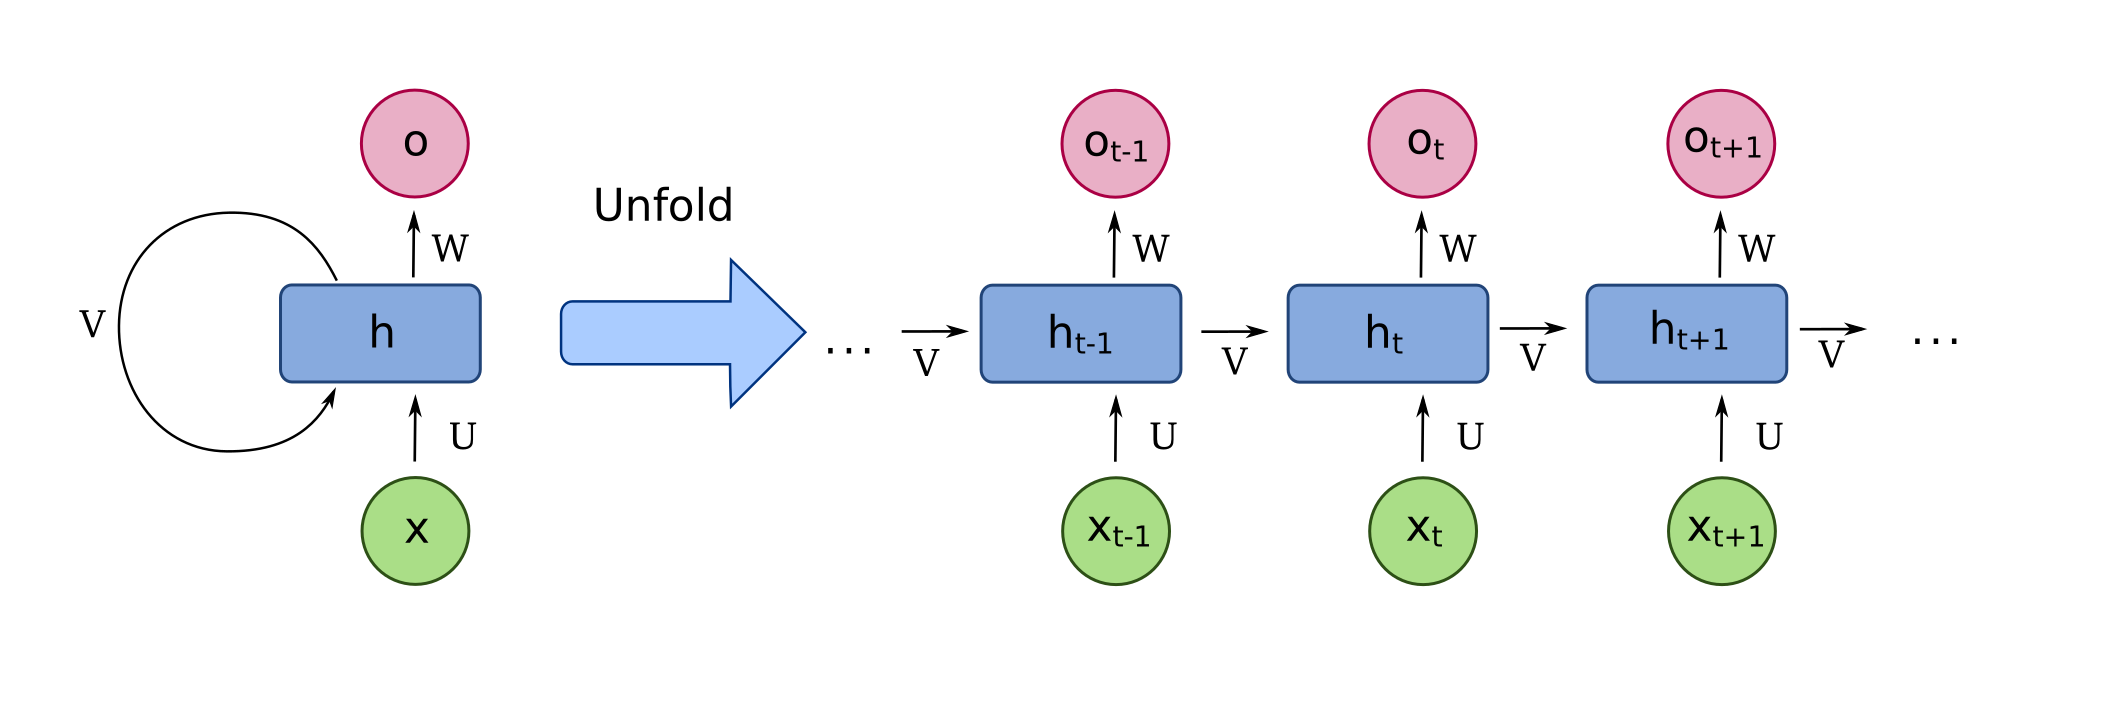
\includegraphics[width=1\textwidth]{images/fully_rnn.png}
    \caption{Basic structure of a fully recurrent neural network.}
    \label{fig:fully_rnn_example}
\end{figure}
A recurrent neural network (RNN) was used because of its capabilities in processing temporal sequence data. This is because this type of artificial neural network has a recurrent architecture, meaning that the output of the previous sample is combined with the input of the current sample \cite{Dupond2019thorough}. The connections of the neurons can be compared to a directed graph. Due to this connectivity, the internal state of the network at a certain point in its training or inference phase can be called memory, because of the still existing output of the previous sample. However, a downside of this architecture is that the previous sample is very present in the 'memory' while earlier samples are increasingly less present. These fully recurrent neural networks therefore have very good short term memory while lacking long term memory (figure \ref{fig:fully_rnn_example}).

Back-propagation (the algorithm used to train artificial neural networks) now has to be performed over time, this is called back-propagation through time (BPTT) \cite{Hochreiter1997long,Robinson1987utility,Werbos1988generalization}. This means that the output of each time step needs to be tracked, which can become quite unwieldy. \textcite{Elman1990finding} found a way around this problem by truncating an unfolded fully RNN to just one time step. This way normal back-propagation can be used again for time sequence data. Elman networks are therefore also called simple recurrent (neural) networks (SRNN). Another type of SRN are Jordan networks \cite{Jordan1997serial}.\\

\subsubsection{(Bi-directional) Long Short-Term Memory Networks}
\begin{figure}[t]
    \centering
    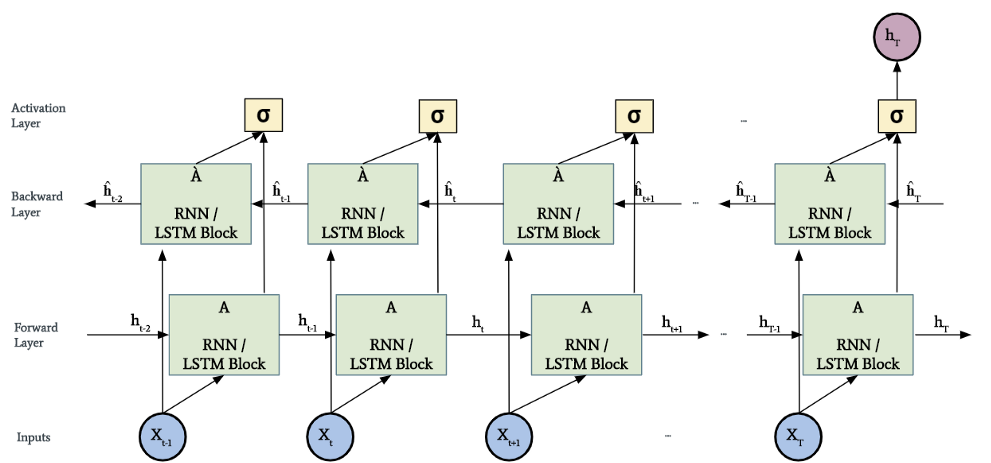
\includegraphics[width=\textwidth]{images/b-lstm}
    \caption{Example Bi-directional long short-term memory neural network with an output state per input and a single output after all inputs are processed.}
    \label{fig:b-lstm}
\end{figure}
As mentioned earlier, SRNN and FRNN suffer from very very good short-term memory while lacking long-term memory. To account for this Long Short-Term memory units were introduced \cite{Hochreiter1997long}. These units were meant to replace the `normal' neurons in a FRNN. LSTM units are different from normal neurons by its inner structure. Normal RNN units work like neurons in a multi-layer perceptron, however instead of only adding up all inputs (or outputs from previous layer), previous outputs are also added to this sum.

A LSTM unit contains an internal state which acts as its memory. An input, output and forget gate decide how the internal state is changed. The way these are set up enables a LSTM to `remember' important data and `forget' less important data of all the data or current input. \textcite{Li2015constructing} found these properties especially suitable for Speech Recognition (`forget' noise, `remember' phonemes), while \textcite{Sak2014long} used these properties for acoustic modeling, because of its performance on time sequence data.

A LSTM network can receives a series of input. The network can then return one output per input sample (sequence-output) or return one output once all inputs are processed (single-output). If one is interested in predicting the word someone is typing, sequence-output can be used. If only the next word needs to be predicted after someone is done typing the previous word, single-output can be used.

A bi-directional (recurrent) neural network, first introduced by \textcite{Schuster1997bidirectional}, is a special kind of recurrent neural networks. A B-RNN works by not only using the input data up to a certain frame, but also the input data from the end to that certain frame. Training thus is performed in both positive and negative time direction. Using both time directions during training enlarges the context of a recurrent unit and was therefore proven to increase the performance of a model. An example of a single-output bi-directional LSTM network can be found in \autoref{fig:b-lstm}.\\

Going back to \citeauthor{Gimeno2020a}; by using a bi-directional RNN with LSTM units, they reported a relative improvement of 19.72\% and 5.35\% compared to the best results in the literature at that moment for their two datasets (Albayzín 2010 and 2012) respectively. 

\subsubsection{Applications of AAS models}
Many applications of models capable of performing such segmentation and classifications are within the broadcast data domain. For example in a live radio broadcast these models can be used to automatically apply the right type of audio filtering onto the broadcast audio stream. This could be an audio filter focused on higher tones when someone is talking or an audio filter focused on lower tones when music is played. Also automatically distinguishing when a person's voice is transmitted through a microphone or background noise, can be used to automatically cut the audio feed of a microphone during a live broadcast.

Non-real time applications of these models are within audio indexing and retrieval of for example documentaries, podcasts or other broadcasts. Audio streams automatically segmented by these models can then be used to speed up the process of retrieving certain parts from documentaries or cut all parts where nobody is talking in a podcast.

By modifying these existing models and extending them from multi-class \textbf{audio} segmentation to multi-class \textbf{music} segmentation will also benefit this field by giving it more specific classes within the music class. Although these models aim to find different kind of patterns within the features used\footnote{I will elaborate on this in the \nameref{sec:acoustic_features} section below.}, the basic principles can be used to decrease the effort needed to create a good performing music segmentation model that uses machine learning.


\section[CNN in MIR]{Convolutional Neural Networks in Music Information Retrieval}
\label{sec:cnn_related}
Another type of machine learning commonly used in another field of computer science and adapted to be useable in \mir\ are Convolutional Neural Networks (CNN). CNN's, first introduced by \textcite{Lecun1989backpropagation} for recognizing handwritten postal codes, and later most improved by \textcite{Krizhevsky2012imagenet}, is a type of artificial neural network that are specialized for processing --most often classifying-- data that has a known grid-like topology. This, as were its first applications, generally is image data, because images have a very well-defined grid-like topology. While binary images being the most simple form of two-dimensional images with for each pixel only 2 possible values, more complex images, like multi-channel images (red-green-blue images, cyan-magenta-yellow-black images) or multi-view images (top view, bottom view, etc,) can be processed too, albeit in a slightly different way.

Convolutional networks are inspired by the neural architecture found in the human visual cortex by \textcite{Hubel1968receptive} in the V1 and V2 area \cite{Lindsay2020convolutional}. Each neuron in the V1 area is sensitive to a sub-region of the visual field, called a \textit{receptive field}. The activation of each neuron then depends on the occurrence of certain visual features (like edges in certain orientations) in the receptive field. The receptive fields are tiled to cover the entire visual field. The current way to imitate this receptive field is to use convolutions, hence the name of this type of artificial neural network. A convolution, or kernel, is a filter that is applied on an image. This way, each neuron in the next layer is connected to a sub-region in the output or image of the layer before (\autoref{fig:cnn_example}). During training, neurons of deeper convolutional layers learn to adapt their weights in such a way that the neuron activates on certain patterns found in the (convolved) image from the layer above, similar to how the neurons in the different visual areas in the visual cortex work.

Feature vectors at first don't seem to be multi-dimensional 'images' however when put in a time sequence one can construct a two-dimensional matrix from multiple one-dimensional feature vectors. This principle makes it possible to also apply convolutional neural networks to natural language processing (NLP) \cite{Lopez2017deep} and music information retrieval. In the case of NLP, each word in a sentence is first converted to a feature vector by either embedding it \cite{Ghannay2016word,Mikolov2013efficient}, or using one hot encoding. The feature vectors of multiple words concatenated then can be used as two-dimensional input for a CNN, slightly imitating the way N-grams work \cite{Brown1992class}.

\textcite{Basili2004classification} were the first to apply machine learning on automatic genre classification of songs. However, they only used Naïve-Bayes, Voting Feature Intervals, Decision Trees and Nearest-Neighbors classifiers. \textcite{Li2010automatic} actually were the first to use convolutional neural networks for automatic genre classification. They were therefore the first to use convolutional neural networks in music information retrieval, and make use of the one-dimensional feature vector concatenation into two-dimensional 'images'. Although they reach over 85\% accuracy when using a dataset with only 3 genres, their accuracy heavily decreases to under 30\% when they use a dataset with 6 genres.
\begin{figure}[t]
    \centering
    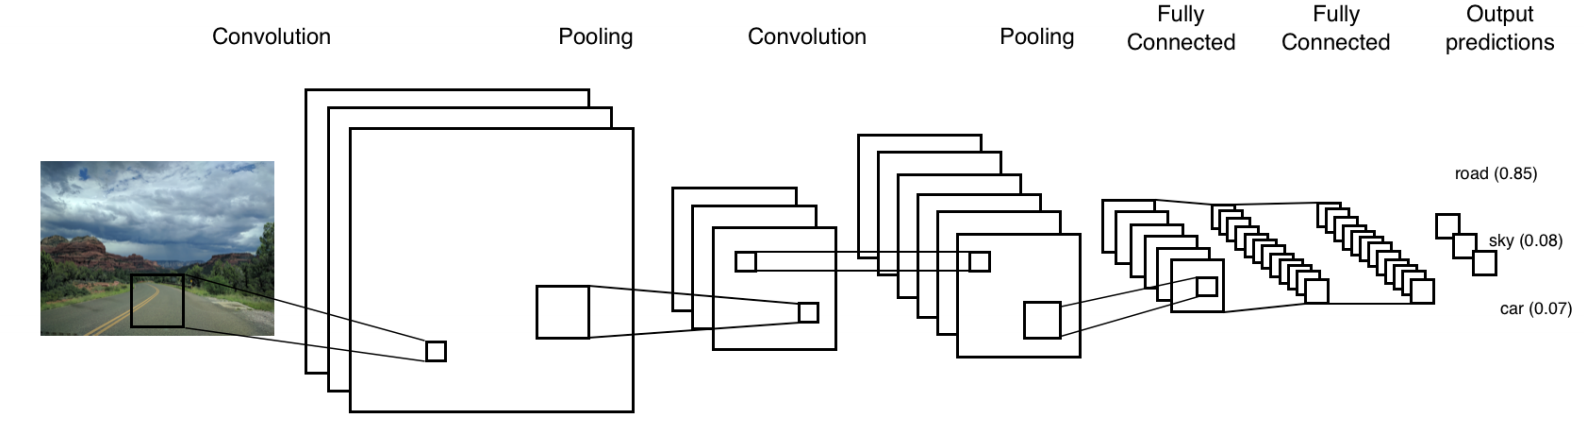
\includegraphics[width=1\textwidth]{images/cnn_example}
    \caption{Basic structure of a convolutional neural network.}
    \label{fig:cnn_example}
\end{figure}

\subsection[CNN for onset detection]{Convolutional Neural Networks for onset detection}
\begin{figure}[t]
    \centering
    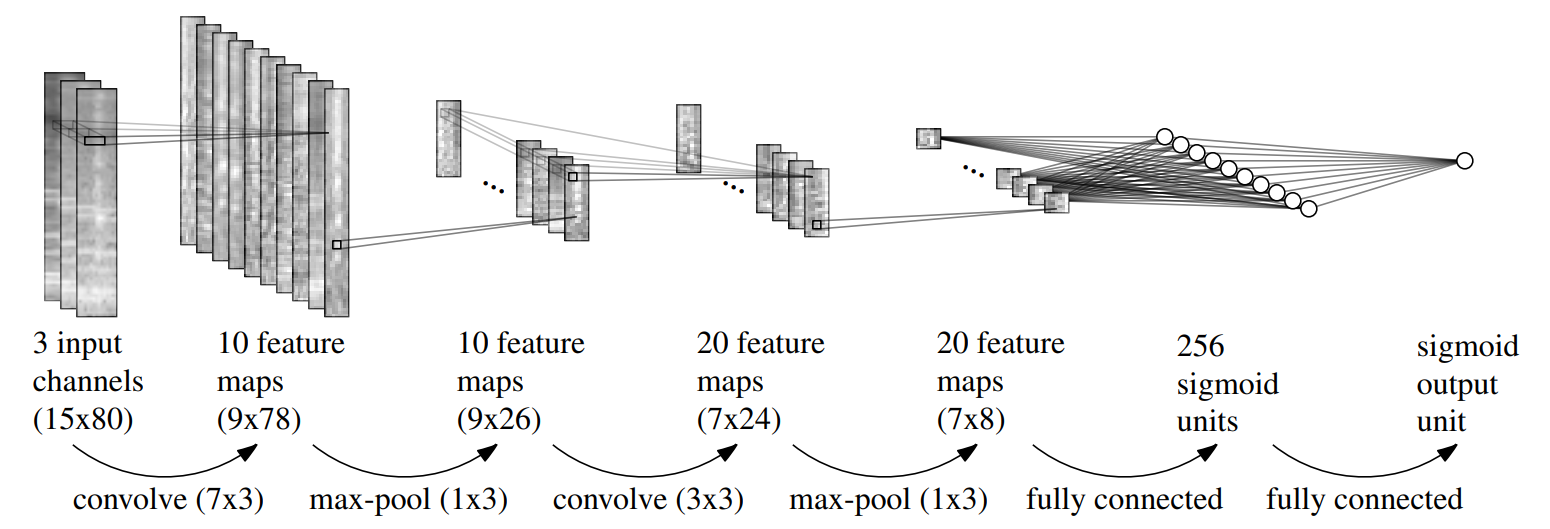
\includegraphics[width=1\textwidth]{images/onset_detection_cnn}
    \caption{Final CNN created for onset detection, starting from a stack of three spectrogram excerpts, ending with one output unit indicating the chance of an onset.\\
    Reprinted from \textcite{Schluter2014improved} (Figure 2).}
    \label{fig:onset_detection_cnn}
\end{figure}
The next subdomain of MIR --related to MSA-- where convolutional neural networks are used with great success, is within musical onset detection.

Musical Onset Detection is the process of automatically extracting the point of time of the musical onsets within a piece of music. A (musical) onset is the beginning of a musical event, most often the beginning of a musical note, but may also be other musical events \cite{Bello2005tutorial,Zhou2011music}. It was first introduced as a contest by Paul Brossier and Pierre Leveau for the MIREX 2005 \footnote{\href{https://www.music-ir.org/mirex/wiki/2005:Audio_Onset_Detect}{See the MIREX website for their proposal. (link)}}. From this moment it has been an annually recurring contest of the MIREX.

Again, using machine learning was on equal performance or outperformed state-of-the-art at that time \cite{Eyben2010universal}. However, in contrast to the current models at that time, this new approach was able to perform real time onset detection by actually predicting the onsets. The proposed model, in multiple ways improved by \citeauthor{Bock2012online}, using a recurrent neural network with long short-term memory (LSTM) units produced a 0.840 F-measure on real time onset detection compared to 0.826 and 0.866 F-measure on non-real time onset detection by state-of-the-art models at that time \cite{Bock2012online}.

After this success with the application of recurrent neural networks for onset detection, \textcite{Schluter2013musical} propose an onset detection method using a convolutional neural network. Not only did this model perform better than the (improved) bi-directional recurrent neural networks at that time (0.885 F-measure compared to 0.873), it also required less (manual) pre-processing, since CNN's are able to 'learn' this pre-processing in their first layer(s). A year later \textcite{Schluter2014improved} report improvements made on the initially proposed model, bringing its F-measure above 0.9 to 0.903 respectively (\autoref{fig:onset_detection_cnn}). \citeauthor{Schluter2014improved} explain the high performance of CNN's on onset detection by their accuracy in finding oriented edges in images. Musical onsets show up as 'edges' in spectrograms of a piece music and a CNN is therefore perfectly suited for finding these edges and thus the onsets\footnote{In practice this is a lot less trivial, however \textcite{Schluter2014improved} have put great effort into trying to explain it.}.

After these successes with the application of CNN's within musical onset detection, \citeauthor{Ullrich2014boundary} made the link to musical structure analysis and its similarity to musical onset detection. Their efforts to also apply convolutional neural networks on this music information retrieval problem resulted in a new state-of-the-art for music structure analysis, which I will describe below.


\section[MSA]{\msa}
Music Structure Analysis, as described in the introduction, is the process of finding important parts in a piece of music, on many possible hierarchical levels. As per my definition I will focus on the functional high level segments in a piece of music. 

In many songs, a few of these high level segments have the same function, and are therefore grouped together. This thus resulted in the two approaches to this problem described in the introduction. Due to the many differences between different songs, even within the same genre, it has always been very difficult to assign a function to a segment. First research to this problem therefore initially focused on finding the segment boundaries first and then group similar segments together. Similar segments were then given the same capital letter denoting their similar function without specifying it further (as verse, chorus, etc.).

\subsection[DSA approach to MSA]{\dsa\ approach to \msa}
\begin{quote}
    \textbf{N.B.} A more in depth overview of the \dsa\ approach can be found in \textcite{Jesperthesis}.
\end{quote}
The DSA approach can be summarized into a few different sub-approaches; a novelty-, homogeneity- and repetition-based approach.

\subsubsection{Self-Similarity Matrix}
\begin{figure}[t]
    \centering
    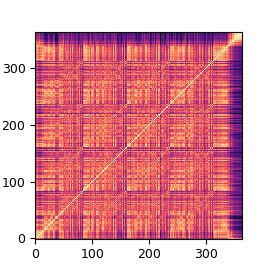
\includegraphics[width=.5\textwidth]{images/ssm}
    \caption{Example of a Self-Similarity Matrix, created on \textit{Mrs. Robinson} by Simon \& Garfunkel.\\
    Reprinted from \textcite{Jesperthesis} (Figure 2.2a).}
    \label{fig:ssm}
\end{figure}
All methods rely on the same main principle, a self-similarity matrix (SSM). A self-similarity matrix, first introduced by \textcite{Foote1999visualizing}, is a matrix calculated by calculating the distance of each feature vector to the other feature vectors. Lower distance values mean that the two feature vectors compared are more similar to each other than two feature vectors with a higher distance value. This will result in a $n\times n$ matrix, where $n$ is the amount of feature vectors of the song. The distances are then normalized to a similarity value. If the distance between two feature vectors is equal to 0, their similarity is equal to 1, all other distance are normalized between a similarity value of 0 and 1. From the way self-similarity matrices are calculated, a diagonal line of similarities with a value of 1 will be seen. This line represents the similarity between each feature vector and itself, which is obviously 1.

\subsubsection{Repetition-based Approach}
The repetition based approach to DSA makes use of this property of SSM's by detecting more diagonal lines in the SSM. Another diagonal line means that a certain part of the song is repeated elsewhere. The start and end of these repetitions can than be used to determine the location of a segment boundary. One technique used to do this is called \textit{Structure Features} \cite{Serra2012unsupervised}. A (cyclic) time lag matrix is constructed from a SSM. This time lag matrix shows horizontal or vertical lines (depending on the exact process used), a line shows for the frame the line occurs in, the amount of time (in frames) it takes before that frame is repeated (in terms of the feature used to create the time lag matrix).

\subsubsection{Novelty-based Approach}
\begin{figure}[t]
    \centering
    \begin{subfigure}{.5\textwidth}
        \centering
        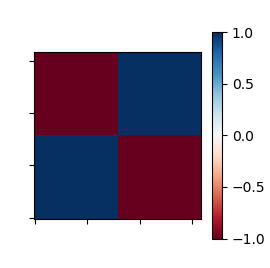
\includegraphics{images/checkerboard}
        \caption{Normal checkerboard kernel}
        \label{pw:fig:foote:norm}
    \end{subfigure}%
    \begin{subfigure}{.5\textwidth}
        \centering
        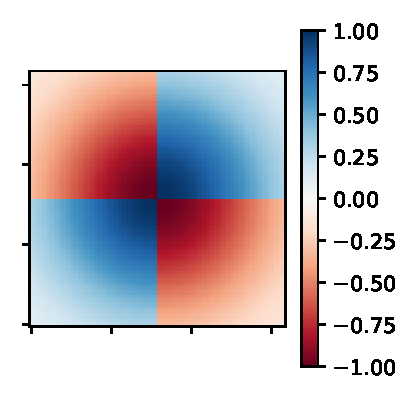
\includegraphics{images/gaussian_checkerboard}
        \caption{Gaussian tapered checkerboard kernel}
        \label{pw:fig:foote:gaus}
    \end{subfigure}
    \caption{An example of a normal and Gaussian tapered checkerboard kernel.\\
    Reprinted from \textcite{Jesperthesis} (Figure 2.3).}
    \label{fig:checkerboard}
\end{figure}
The novelty based approach makes use of another property of SSM's: blocks. A block in a SSM denotes a section of consistent features for the duration of the block. \textcite{Foote2000automatic} was the first to come up with a way to detect the transition of one block into another along the main diagonal of the SSM. Their method used a (Gaussian) checkerboard kernel. A most basic checkerboard kernel can be constructed using a $2\times2$ matrix, like this:
$$\mathbf{K} = \begin{bmatrix} -1 & 1 \\ 1 & -1 \end{bmatrix}$$
It functions similar to how a \textit{Sobel Operator} works in image processing to detect edges. However, where the \textit{Sobel Operator} uses a horizontal and vertical operator to detect horizontal and vertical edges, a checkerboard kernel is specifically designed to detect diagonal edges.

Since this is a $2\times2$ matrix, only 2 different feature vectors will be taken into account, it is therefore more common in music structure analysis to use larger checkerboard kernels, like $64\times64$. To give more importance to closer feature vectors, the checkerboard matrix can be tapered with a Gaussian function (\autoref{fig:checkerboard}).

By applying a checkerboard kernel over the diagonal of a SSM, an 'edge activation' can be calculated for each feature vector. From this a \textit{novelty curve} can be constructed, denoting the amount of novelty (in terms of the acoustic features used) between two adjacent feature vectors. By, for example, applying adaptive thresholding, the peaks in this novelty curve can be extracted. The location of each peak then stands for the location of a segment boundary.

\subsubsection{Homogeneity-based Approach}
The homogeneity-based approach to DSA has been researched a lot less. A most recent research implements this approach using a Hidden Markov Model. Each state stands for a homogeneous piece of music, and the chance to go to the next state determines the chance of a segment boundary.

\subsubsection{2D fourier Magnitude Coefficients}
Once all segment boundaries are detected, the segments can be extracted. Then all segments need to be labeled. One of the most common ways is to use some kind of clustering method, and then assigning a label to each cluster. Each segment, however, can be of different length. A way to represent each segment in such a way that a distance metric could be applied was therefore needed. The use of the magnitude of the 2D Fourier Transform, originally a technique used in image processing, was therefore first introduced by \textcite{Ellis2007beat}. \textcite{Nieto2014music} were the first to apply the 2D Fourier Magnitude Coefficients for segment clustering.

Clustering segments this way proved to be quite accurate. One big problem however, was the amount of clusters that had to be used, since this could vary per song.

\subsection{Current State-of-the-Art}
\begin{figure}[t]
    \centering
    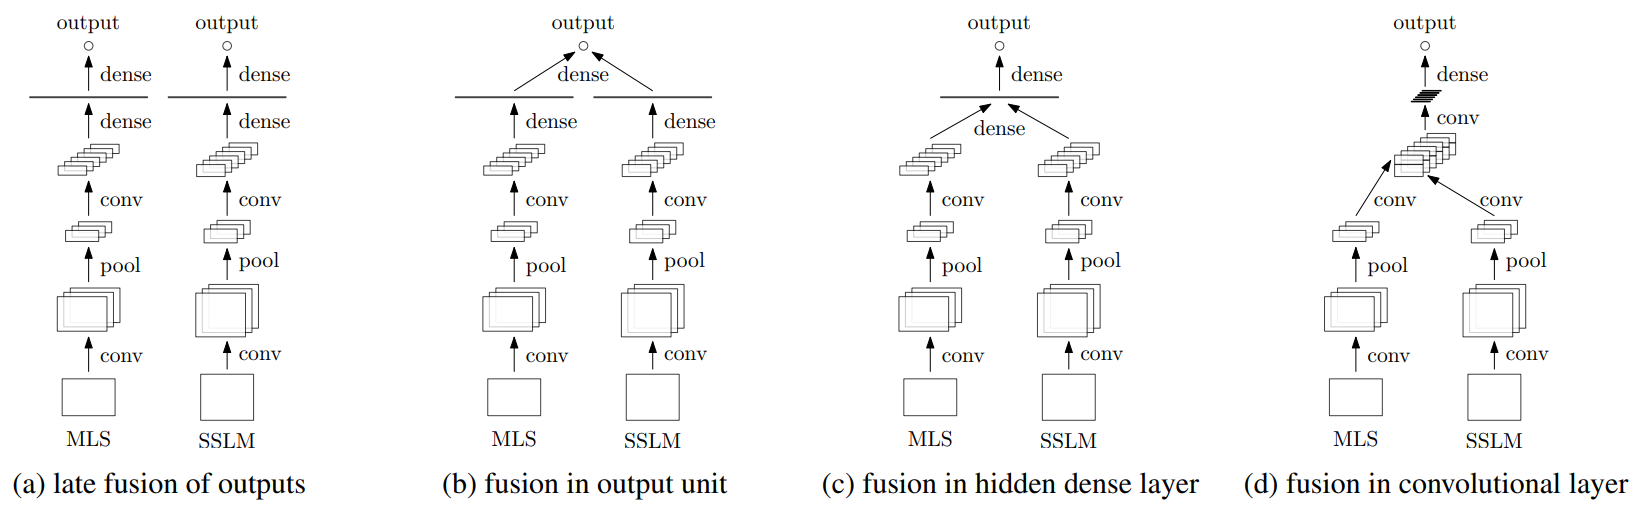
\includegraphics[width=1\textwidth]{images/fusion_examples_cnn}
    \caption{Four different CNN architectures for combining two input features.\\
    Reprinted from \textcite{Grill2015music}.}
    \label{fig:fusion_examples_cnn}
\end{figure}
Due to the successes of CNN's within onset detection and its similarity to finding the segment boundaries --the start of a new high level segment can be compared to a strong onset viewed in a big time window-- , \citeauthor{Ullrich2014boundary} therefore put their effort into creating a convolutional network that is capable of finding these boundaries, based on their model created for onset detection. They presented their first results in \citeyear{Ullrich2014boundary} \cite{Ullrich2014boundary}. They report an advance of state-of-the-art of that time for MSA, F-measure of 0.33 to 0.46 for 0.5s tolerance and F-measure of 0.52 to 0.62 for 3s tolerance.\footnote{A 0.5 or 3 second tolerance means that a segment boundary is counted as a hit if it lies within 0.5 or 3 seconds of the ground truth. Refer to \textcite{Jesperthesis} (section 2.2.2) for more elaboration on this subject.} A few different input features were tested (MFCC, Chroma, Mel spectrograms), and finally 5 different models trained on Mel spectrograms were bagged \cite{Breiman1996bagging} together for their final model.

To account for misses of boundaries between non-local musical cues, such as segment repetitions, \textcite{Grill2015music} present an improvement on the initial convolutional network by combining the Mel-scaled Log-magnitude Spectrograms (MLS) with Self-Similarity Lag Matrices (SSLM) as input. They test different models that each combine these inputs at a different moment in the model (\autoref{fig:fusion_examples_cnn}). Their best model, fusing the inputs in the convolutional layer (\autoref{fig:fusion_examples_cnn}d), advanced the F-measure from 0.46 \cite{Ullrich2014boundary} to 0.52.

\textcite{Grill2015music2} further expanded this model by dividing the SSLM into a near (14 second time context) and far (88 second time context) variant, each used as different feature combined with a MLS as their input for their models. They also added another neuron to the output layer giving it two neurons in total. One of these neurons was trained on lower level annotation available in their dataset, while the other neuron was trained on the high level annotation. They show that using two annotation levels increases the F-measure of over 0.3 on 0.5s tolerance.

They present their final model in their MIREX submission for the MIREX 2015 Music Structural Segmentation task \cite{Grill2015structural}.


\section{SALAMI Dataset}
\label{sec:salami}
Many datasets have been created and used for music structure analysis. An extensive listing with most well-known data-sets can be found on \href{https://ismir.net/resources/datasets/}{the website of the International Society of Music Information Retrieval (ISMIR)}. There are a total of 16 data-sets listed there that cover musical structure. Only 5 of these data-sets cover western popular music and feature a song total above 100, these are the INRIA:Eurovision, INRIA:Quaero, QMUL:Beatles, RWC and SALAMI datasets respectively.\\
Although these datasets contain the annotations, and some of them also the features, of the songs, none of these actually provide the audio of the annotated songs.\\
The only dataset that did provide a link to the audio files is the SALAMI dataset. The SALAMI dataset, or \textit{Structural Analysis of Large Amounts of Musical Information} dataset, is an unprecedented large dataset that contains 2400 structural annotations \cite{Salami}. This dataset contains, among many other subsets, an \textit{internet archives} subset. The internet archives subset contains the annotations of songs publicly available on the internet together with a link to an mp3 file with the audio.


\section{Acoustic Features}
\label{sec:acoustic_features}
To represent the audio in a more meaningful way, many features have been used or proposed in the past, in this section I will inspect a few of most popular features that are being used or have been used in music information retrieval and music structure analysis in particular. Further explanation of these features among citations to great other sources about these features can be found in \cite{Paulus2008acoustic}.

\subsection{Chroma}
\begin{figure}[t]
    \centering
    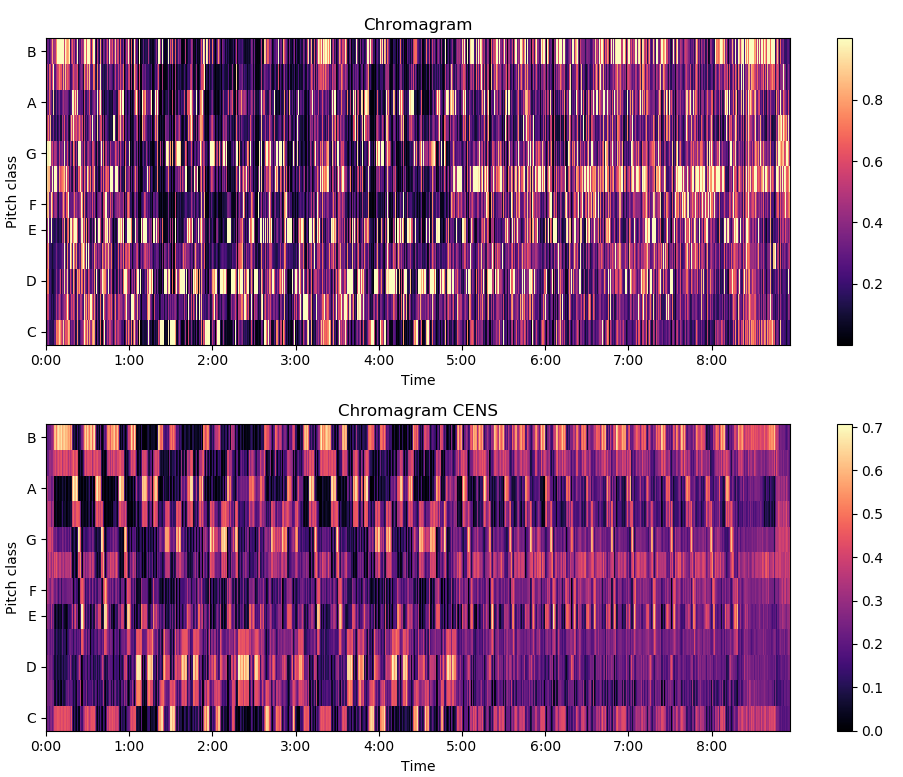
\includegraphics[width=\textwidth]{images/cqt_cens}
    \caption{PCP chromagram compared to CENS chromagram, both constructed with 12 bins, 2048 FFT window size and 512 hop length.}
    \label{fig:pcp_cens}
\end{figure}
The chroma, or 'color', of a song closely relates to the (often twelve) different pitch classes in music. There are multiple chroma types, each one calculated in a different way to represent each pitch class in a slightly different way. The first step for each chroma type however, is to first create a \textit{spectrogram}. A spectrogram is created by applying the discrete fourier transform (DFT) on a slice, or \textit{window}, of the audio. By repeatedly applying the DFT on the window, while it is being slid or hopped through the audio, one can create a representation of the intensity of each frequency over time. This technique is called the \textit{Short Time Fourier Transform} (STFT). 

The window size in this context is called the Fast Fourier Transform or \textbf{FFT window size} (often 2048 or 4096 audio samples). Each time the window is moved, the amount of audio samples it moves is called the \textbf{hop length} (often 512 or 1024). If a FFT window size of 4096 is used and a hop length of 1024, one can see that there is 75\% overlap between each output of the DFT.

The \textit{Pitch Class Profile} (PCP) \cite{Lee2006automatic} is one of the most low-level chroma representations. The STFT spectrogram is converted to an intensity of each 12 pitch classes ($C$, $C\sharp$, $D$, etc.) on the equal-tempered scale. If 12 bins are used, each bin represents a semitone, if a multiple of 12 bins are used, each bin represents an equal fraction of a semitone. The PCP has primarily been used to compute the similarity between two songs, however more computation and analysis is needed to extract higher-level patterns from the PCP.

The \textit{Chroma Energy Normalized Statistics}, or CENS, chroma representation \cite{Muller2005chroma} is another chroma representation commonly used in audio matching, audio retrieval and music similarity. This feature is more popular in this fields because of its robustness to audio dynamics, timbre and articulation. This robustness is obtained by taking statistics over large windows, therefore smoothing local deviations in tempo, articulation and music ornaments such as trills and arpeggiated chords. A downside to this smoothing is that at some points in time it can be hard to determine which pitch class is the most dominant.

A comparison between a PCP chromagram and CENS chromagram can be found in \autoref{fig:pcp_cens}.

\subsection{Timbre}
\begin{figure}[t]
    \centering
    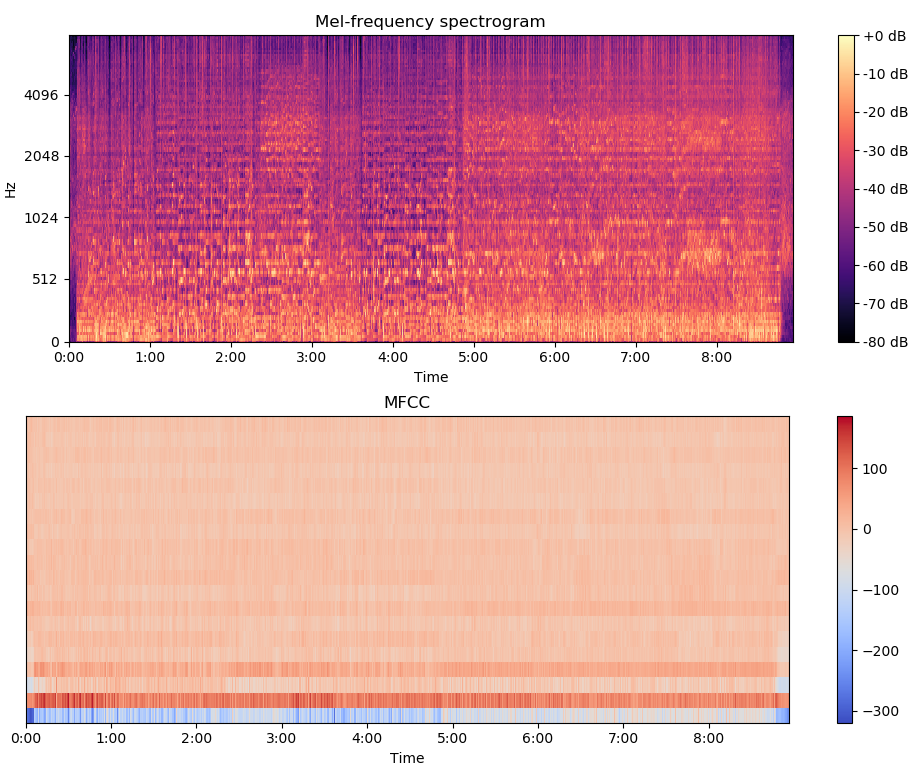
\includegraphics[width=\textwidth]{images/mls_mfcc}
    \caption{Mel-frequency spectrogram compared to Mel Frequency Cepstral Coefficients with 20 bins.}
    \label{fig:mls_mfcc}
\end{figure}
Another way of representing audio is by its timbre. Timbre has no direct definition, it however is generally described as \textit{'The perceived sound quality of a musical note, sound or tone'}. Timbre was introduced to distinguish between two instruments, since two instruments playing the same tone, will have the same chroma value.

While the Fourier Transform is able to extract the intensity of each frequency, it has a few flaws. That is why the Mel Scale was created. The mel scale, originally introduced by \textcite{Stevens1937scale}, is a perceptual scale that scales each pitch judged by listeners to be in equal distance from each other. They introduced this scale because the human auditory system is not equally sensitive to each audio frequency, for example the human auditory system is most sensitive to the 2000 to 5000 Hz range \cite{Gelfand1997essentials}, while the screams of a baby are around the 3500 Hz region. 

Using the mel scale we can create so-called Mel-scaled spectrograms, or cepstrograms, that represent the intensity of each mel-frequency at each audio sample. A cepstrogram does represent the different sounds quite good, especially since the vector length at each time point is a lot longer than 12 (or a low factor of thereof). However, due to its enormous dimensions, using a cepstrogram as feature for a model can be quite computational intensive.

Partly for this reason, the \textit{Mel Frequency Cepstral Coefficients} (MFCC) were created \cite{Logan2000mel}. The MFCC discretize a mel-scaled spectrogram by first taking the Fourier Transform of an audio stream. Then, the powers of the spectrum is mapped onto the mel-scale, using triangular overlapping windows. The log of the power of each mel frequency is taken, followed by a discrete cosine transform over the list of mel log powers. Often 20 bins are used for the final vector length of the MFCC. A comparison between a mel-scaled spectrogram and the MFCC of that same spectrogram can be found in \autoref{fig:mls_mfcc}.

Although its high information density, MFCCs are not 'the ultimate feature to describe all audio' \cite{Pachet2004improving}. Therefore, other timbre features still need to be considered, one example being the \textit{Constant-Q Transform} (CQT) \cite{Brown1991calculation}. The CQT is very closely related, but is calculated in a slightly other way. However, due to the complex calculation, another way of calculating the CQT using the FFT in conjunction with a kernel was proposed \cite{Brown1992efficient,Blankertz2001constant}.

\subsubsection{Rythm}
\begin{figure}[t]
    \centering
    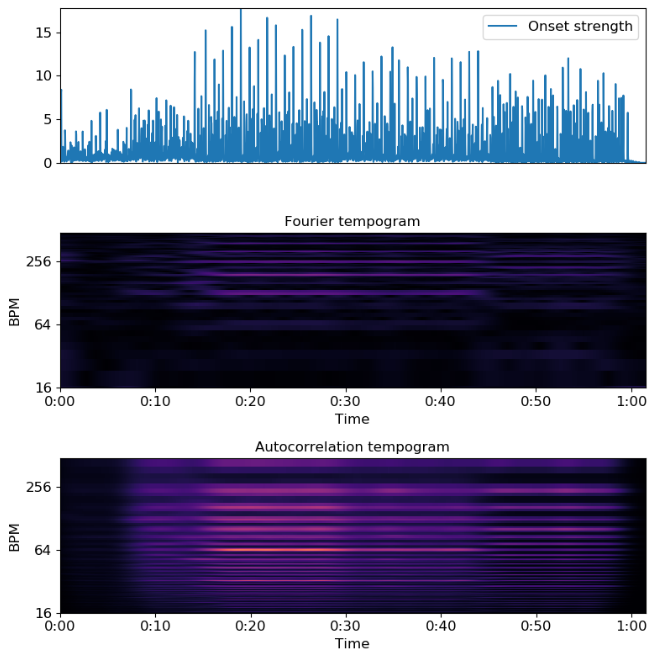
\includegraphics[width=\textwidth]{images/tempogrammi}
    \caption{A comparison of a Fourier tempogram and autocorrelation (cyclic) tempogram made on the same onset strength envelope.}
    \label{fig:tempogrammi}
\end{figure}
Not only the tones or harmony of a piece of music can be used as input for music information retrieval models, rhythmic features can also add a lot of information. This is especially applicable to the detection of the musical structure. Similar segments often employ similar rhythmic features, while different segments, like verse and chorus, can differ a in their rhythmic. Rhythmic features therefore can be used to both label or cluster segments. or to detect boundaries between two segments (when a sudden change in a rhythmic feature is detected).

One of the most well known rhythmic features will be tempo. Tempo can be represented as the amount of beats per minute (BPM). Tempo represented on a time scale is called a \textit{tempogram}; the feature vector at each time point represents the probabilities of a certain BPM at that time point. 

Since detecting the tempo at each time point turned out to be quite difficult, cyclic tempograms were introduced \cite{Grosche2010cyclic}. A cyclic, or autocorrelation, tempogram detects tempi differing with a power of two, thereby reducing the amount of possible tempi at a certain time point, and thus increasing the probability value of the most probable tempo, since there will be more tempi differing with a power of two around the true tempo.

Another way of computing a tempogram is by using a (short-time) Fourier transform on the onset strength envelope. A comparison between these tempograms can be found in \autoref{fig:tempogrammi}.